\chapter{Resultados y conclusiones.}

\section{Comparaci\'on TIF.}

\hspace{0.4cm} La comparaci\'on de los precios te\'oricos obtenidos mediante el uso de la metodolog\'ia de los Splines c\'ubicos de suavizado con la metodolog\'ia Svensson para los Tif, se presenta a continuaci\'on en la Tabla \ref{tabla2}.

\renewcommand{\tablename}{Tabla}
\begin{table}[H]
\centering
%\begin{center}
\scalebox{0.85}{\begin{tabular}[t]{|c |c |c |c |c |c |r|}
\hline
T\'itulo & Precio Promedio & Precio Splines & Precio Svensson & Precio Svensson Optimizado  \\
\hline
TIF082018 & 101,00 & 107,27 & 107,35 & 100,92  \\
\hline
TIF042019 & 112,00 & 116,38 & 119,48 & 113,41  \\
\hline
TIF082019 &  110,00& 109,42 & 112,81 & 108,19 \\
\hline
TIF112020 & 130,02 & 127,62 & 130,15 & 127,28  \\
\hline
TIF022021 & 129,01 & 128,05 & 130,37 & 127,56  \\
\hline
TIF042023 & 128,10 & 132,21 & 134,03 & 130,27  \\
\hline
TIF012024 & 120,00 & 134,42 & 136,25 & 132,02 \\
\hline
TIF062025 & 124,00 & 130,44 & 131,61 & 126,85  \\
\hline
TIF012026 & 122,00 & 130,31 & 131,05 & 126,04  \\
\hline
TIF112027 & 126,52 & 132,04 & 130,75 & 125,08 \\
\hline
TIF032028 & 128,52 & 135,83 & 134,02 & 128,15  \\
\hline
TIF052028 & 128,19 & 137,56 & 131,76 & 125,88  \\
\hline
TIF032029 & 132,03 & 140,30 & 137,37 & 131,18  \\
\hline
TIF022030 & 128,52 & 142,86 & 138,91 & 132,42  \\
\hline
TIF022031 & 130,10 & 135,95 & 131,54 & 125,01  \\
\hline
TIF032031 & 128,53 & 138,30 & 133,87 & 127,30  \\
\hline
TIF022032 & 127,00 & 135,13 & 127,48 & 120,92\\
\hline
TIF032032 & 128,52 & 139,45 & 135,46 & 128,60  \\
\hline
TIF032033 & 127,01& 135,37 & 130,67 & 123,91\\
\hline
TIF052034 & 127,12 & 128,51 & 124,08 & 117,35\\
\hline
Error & NA & 4,6224 & 5,2694 & 0,3610\\
\hline
\end{tabular}}
%\end{center}
\caption{Comparaci\'on precios TIF.}
\label{tabla2}
\end{table}


\hspace{0.4cm} Para la creaci\'on de la tabla anterior, se consideraron los siguientes par\'ametros,

\begin{itemize}
  \item Fecha de valoraci\'on: $08/03/2018$.
  \item D\'ias hacia atras: 40.
  \item Par\'ametro de suavizamiento: 0.2
\end{itemize}


\hspace{0.4cm} En la tabla anterior se observan los precios promedios de cada instrumento para el a\~no en curso, los precios te\'oricos obtenidos mediante la metodolog\'ia de Splines y los precios te\'oricos obtenidos mediante la metodolog\'ia de Svensson, en este caso se tienen dos resultados uno es usando unos par\'ametros por defecto (Columna Precio Svensson) y el otro es usando el proceso de optimizaci\'on para esta metodolog\'ia. En la \'ultima fila se observa el valor de la suma del error cuadr\'atico (Error), el cual se obtiene luego de realizar la suma de los cuadrados de las diferencias que existen entre el precio te\'orico de cada instrumento y su precio promedio. Mientras mas peque\~no sea este valor m\'as se asemejar\'an los precios te\'oricos a los precio promedio.

\hspace{0.4cm} Si se comparan los precios te\'oricos obtenidos mediante la metodolog\'ia de Splines y aquellos obtenidos mediante la metodolog\'ia de Svensson (sin optimizar), se puede afirmar que mediante la primera metodolog\'ia se obtiene una mejor aproximaci\'on de dichos precios con respecto a los precios promedio de cada instrumentos esto debido al Error que para el caso de los Splines es de $4.6224$, mientras que para el caso de Svensson es de $5.2694$.

\hspace{0.4cm} Por su parte, si se observa el error obtenido para la metodolg\'ia de Svensson optimizada ($0.3610$), este valor es mucho m\'as peque\~no que las dos metodolog\'ias anteriores, esto se debe al proceso de optimizaci\'on ya que en el mismo se busca que esta diferencia sea m\'inima.

\hspace{0.4cm} La Figura \ref{curva_spline_tif}, muestra la curva de rendimiento para los TIF obtenida mediante el ajuste del Spline de suavizado, por su parte la nube de puntos fue obtenida a partir de la base de datos de estos instrumentos para la cantidad de d\'ias seleccionado, en este caso 40. Estos puntos representan los rendimientos obtenidos a partir de las operaciones realizadas con estos instrumentos en el horizonte temporal considerado. El eje x de la gr\'afica muestra la maduraci\'on en d\'ias, por su parte el eje y muestra el rendimiento estimado.

\newpage

\section{Comparaci\'on VEBONO.}


\hspace{0.4cm}La siguiente tabla muestra los resultados de los precios te\'oricos obtenidos para los Vebonos mediante las diferentes metodolog\'ias consideradas. Para la creaci\'on de la misma, se consideraron los siguientes par\'ametros,

\begin{itemize}
  \item Fecha de valoraci\'on: $08/03/2018$.
  \item D\'ias hacia atras: 40.
  \item Par\'ametro de suavizamiento: 0.4
\end{itemize}

%\begin{center}
\begin{table}[H]
\centering
\scalebox{0.90}{\begin{tabular}[t]{|c |c |c |c |c |c |r|}
\hline
T\'itulo & Precio Promedio & Precio Splines & Precio Svensson & Precio Svensson Optimizado  \\
\hline
VEBONO072018 & 100,40 & 106,17 & 108,14 & 100,41  \\
\hline
VEBONO022019 & 106,00 & 107,75 & 111,18 & 104,98  \\
\hline
VEBONO032019 &  110,00& 113,55 & 117,10 & 111,38 \\
\hline
VEBONO012020 & 121,00 & 118,42 & 121,05 & 118,92  \\
\hline
VEBONO062020 & 127,83 & 120,97 & 122,60 & 122,23  \\
\hline
VEBONO012021 & 130,32 & 121,96 & 122,27 & 123,36  \\
\hline
VEBONO052021 & 127,00 & 122,01 & 121,72 & 123,28 \\
\hline
VEBONO122021 & 129,45 & 126,18 & 124,86 & 126,88  \\
\hline
VEBONO022022 & 129,00 & 123,15 & 121,55 & 123,62 \\
\hline
VEBONO012023 & 129,96 & 126,79 & 123,69 & 125,78 \\
\hline
VEBONO022024 & 128,00 & 128,27 & 123,88 & 125,77  \\
\hline
VEBONO022025 & 128,50 & 134,25 & 125,35 & 126,96  \\
\hline
VEBONO042028 & 129,68 & 132,08 & 127,80 & 128,62  \\
\hline
VEBONO102028 & 130,01 & 131,67 & 127,68 & 128,40  \\
\hline
VEBONO052029 & 125,03 & 131,16 & 127,26 & 127,91  \\
\hline
VEBONO102029 & 125,75 & 132,32 & 128,24 & 128,79 \\
\hline
VEBONO072030 & 130,50 & 132,44 & 127,72 & 128,16\\
\hline
VEBONO062032 & 128,53 & 128,07 & 121,73 & 121,89  \\
\hline
VEBONO072033 & 130,00& 127,31 & 120,40 & 120,45\\
\hline
VEBONO022034 & 128,02 & 126,53 & 119,49 & 119,51\\
\hline
Error & NA & 3,5817 & 6,7379 & 0,3608\\
\hline
\end{tabular}}
%\end{center}
\caption{Comparaci\'on precios VEBONO.}
\label{tabla3}
\end{table}

\newpage

\hspace{0.4cm} Al igual que en la tabla comparativa para los TIF, la Tabla \ref{tabla3} muestra los precios te\'oricos obtenidos por tres metodolog\'ias, la primera la de Splines de suavizaso, la segunda la de Svensson sin optimizar y finalmente la tercera, la de Svensson optimizado. Estas metodolog\'ias, son comparadas con los precios promedio para cada instrumento.

\hspace{0.4cm} Si se compara los precios te\'oricos obtenidos mediante la metodolog\'ia de Splines de suavizados con los precios obtenidos mediante la metodolog\'ia de Svensson sin optimizar, podemos decir que los primeros muestran un mejor comportamiento al ser comparados con los precios promedio de cada t\'itulo valor. Esto debido a que el error obtenido es menor.

\hspace{0.4cm}Por otra parte, si estos precios son comparados con los obtenidos mediante la metodolog\'ia de Svensson optimizada, se observa que estos \'ultimos poseen un excelente comportamiento, ya que su error es bastante peque\~no. En la Figura \ref{curva_spline_veb} se observa la curva de rendimientos obtenida para la fecha de valoraci\'on y cantidad de d\'ias seleccionado. En este caso la nube de puntos, al igual que para los TIF surgue de la base de datos de las operaciones m\'as recientes transadas con este tipo de instrumentos.

\subsection{Curvas de Rendimiento.} \hspace{5cm}


\begin{figure}[h]
  \scalebox{0.80}{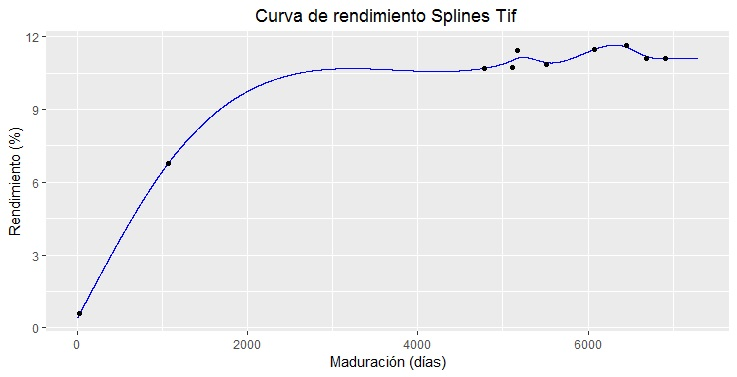
\includegraphics{images/c_tif.jpg}}
%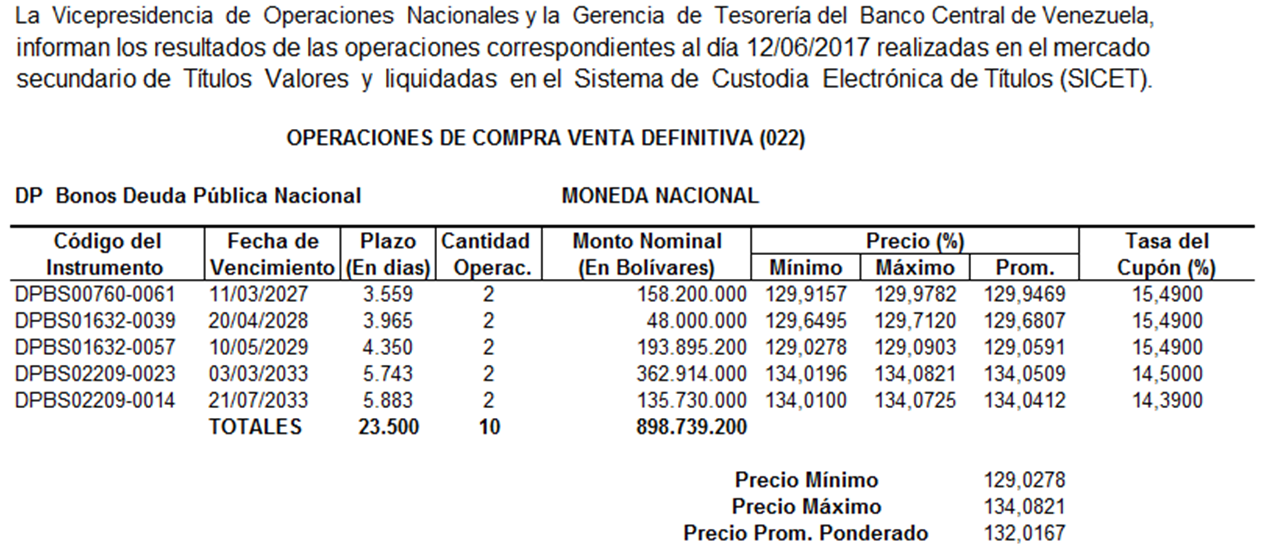
\includegraphics[width=0.7\textwidth]{Imagen022.png}
\caption{Curva Spline TIF.}
\label{curva_spline_tif}
\end{figure}


\begin{figure}[h]
  \scalebox{0.80}{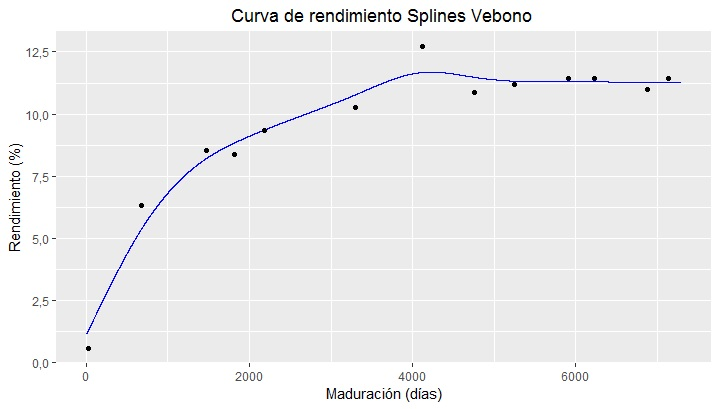
\includegraphics{images/c_veb.jpg}}
%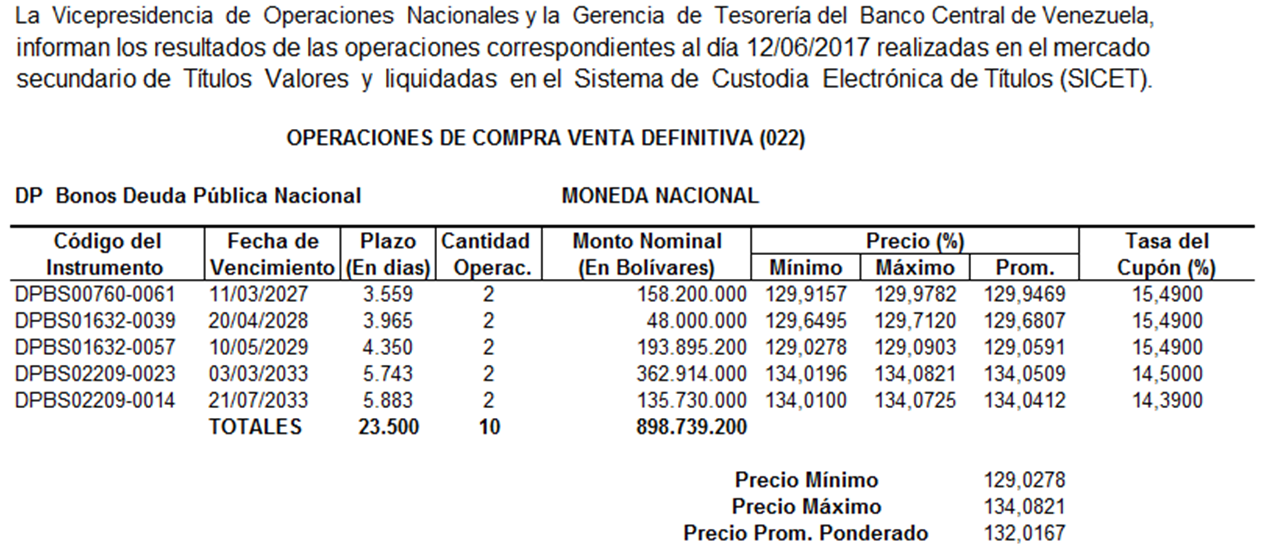
\includegraphics[width=0.7\textwidth]{Imagen022.png}
\caption{Curva Spline VEBONO.}
\label{curva_spline_veb}
\end{figure}

\newpage

\section{Comparativo curvas de Rendimiento.}

\hspace{0.4cm} En las Figuras \ref{curva_spline_comp_tif} y \ref{curva_spline_comp_veb} , se muestra una comparaci\'on entre las curvas de rendimiento obtenidas mediante la metodolog\'ias de Splines de suavizado, Svensson sin opmitizar y Svensson Optimizado.
Para el caso de la metodolog\'ia de los Splines se us\'o un par\'ametro de suavizamiento de 0.2 para los TIF y 0.4 para los Vebono, recordemos que este factor controla la suavidad de la curva obtenida. Por su parte las curvas obtenidas para las metodolog\'ias de Svensson optimizada y sin optimizar surgen de los par\'ametros considerados al momento de calcular los precios te\'oricos de los instrumentos.

\hspace{0.4cm}Recordemos que para la metodolog\'ia Svensson sin optimizar se usaron unos par\'ametros por defecto, mientras que para la metodolog\'ia de Svensson optimizada se usaron aquellos par\'ametros de minimizaran la diferencia entre los precios te\'oricos y los precio promedio. La Tabla \ref{tabla4} muestra una comparaci\'on con estos valores para el caso de los TIF .

\begin{table}[H]
\centering
{\begin{tabular}[t]{|c |c |c |c |c |c |c |c |r|}
\hline
Metodolog\'ia / Par\'ametro / TIF & $\beta_{0}$ & $\beta_{1}$ & $\beta_{2}$ & $\beta_{3}$  &  $\tau_{1}$ & $\tau_{2}$ \\
\hline
Svensson sin optimizar & 0,1337 & -0,0100 & -0,3078 & -0,1340  & 0,5453 & 0,3506\\
\hline
Svensson Optimizado & 0,1430 & 0,2119 & -0,6438 & 0,3327 & 0,5744 & 0,0184 \\
\hline
\end{tabular}}
\caption{Par\'ametros Svensson TIF.}
\label{tabla4}
\end{table}


\newpage

\begin{figure}[h]
  \scalebox{0.65}{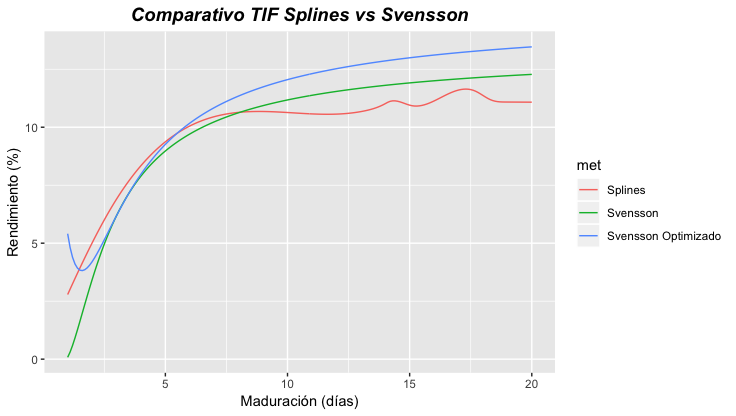
\includegraphics{images/Comparativo_tif.png}}
%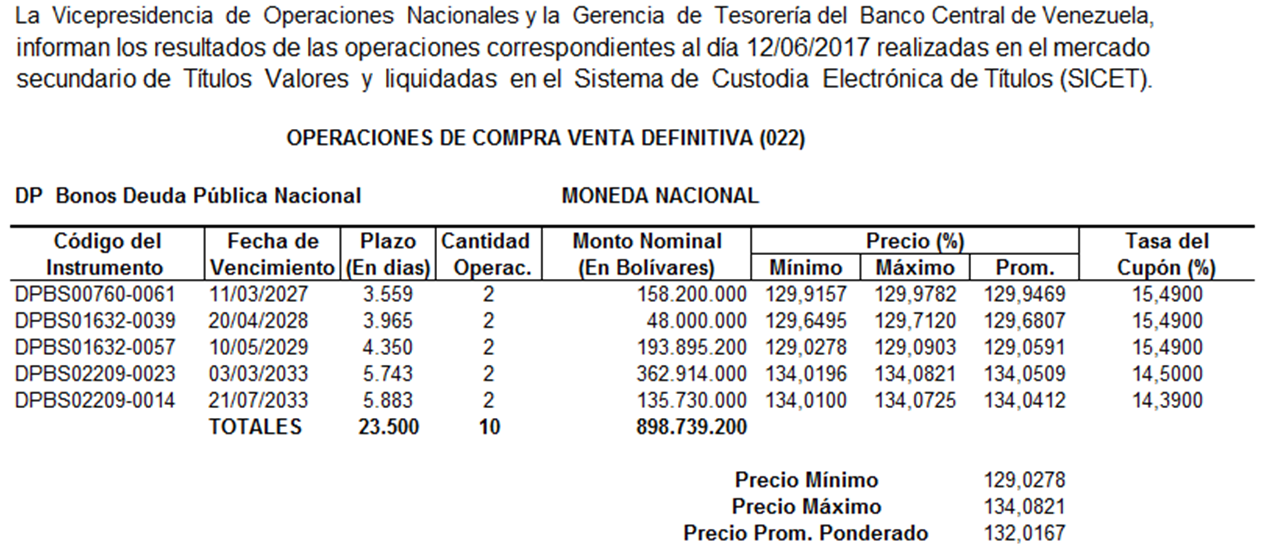
\includegraphics[width=0.7\textwidth]{Imagen022.png}
\caption{Curva TIF Spline vs Svensson.}
\label{curva_spline_comp_tif}
\end{figure}

\hspace{0.4cm} En la Figura \ref{curva_spline_comp_tif} se aprecia que la curva obtenida mediante la metodolog\'ia de los splines c\'ubicos de suavizado (curva roja) resulta ser la curva que menos altura alcanza en promedio siendo su valor m\'aximo $12 \%$, lo cual influye directamente en los precios obtenidos, esto debido a la relaci\'on inversa que existe entre el rendimiento y el precio de un instrumento. En este caso, al obtenerse rendimientos relativamente bajos se obtendr\'an precios relativamente elevados. 

\hspace{0.4cm} Por su parte si se observa la curva de rendimientos obtenida mediante la metodolog\'ia de Svensson sin optimizar (curva verde), la misma presenta alturas m\'as grandes que la curva anterior, alcanzando su m\'aximo en $12,5 \%$. Esto ocasiona, que para esta metodolog\'ia se obtengan precios un tanto m\'as bajos.

\hspace{0.4cm} Finalmente si se observa la curva de rendimientos obtenida mediante la metodolog\'ia de Svensson optimizada (curva azul), vemos que ella presenta las alturas m\'as elevadas, alcanzando su valor m\'aximo en $13 \%$ . De esta manera, los precios a obtener ser\'an m\'as bajos y en este caso los precios que m\'as se asemejan a los precios te\'oricos de los instrumentos TIF.




\newpage

\hspace{0.4cm} La tabla \ref{tabla5} muestra los par\'ametros utilizados para elaborar las curvas de rendimientos para el caso de la metodolog\'ia de Svensson sin optimizar y Svensson optimizado. Es importante destacar, que cada par\'ametro controla una secci\'on de la curva.

\begin{table}[H]
\centering
{\begin{tabular}[t]{|c |c |c |c |c |c |c |c |r|}
\hline
Metodolog\'ia / Par\'ametro / VEBONO & $\beta_{0}$ & $\beta_{1}$ & $\beta_{2}$ & $\beta_{3}$  &  $\tau_{1}$ & $\tau_{2}$ \\
\hline
Svensson sin optimizar & 0,1358 & 0,1000 & -0,5037 & -0,2887 & 0,1195 & 0,5017\\
\hline
Svensson Optimizado & 0,1421 & 0,4845 & -0,4343 & -0,3514 & 0,1985 & 0,7851 \\
\hline
\end{tabular}}
\caption{Par\'ametros Svensson VEBONO.}
\label{tabla5}
\end{table}

\vspace{0.5cm}

\hspace{0.4cm} La Figura \ref{curva_spline_comp_veb} muestra una comparaci\'on entre las curvas obtenidas por las tres metodolog\'ias consideradas. La curva roja muestra la curva de rendimientos obtenida mediante la metodolog\'ia de Splines c\'ubicos de suavizado, la misma presenta ciertas ``jorobas", las cuales son ocasionadas por las observaciones obtenidas para el per\'iodo de estudio considerado. Esta curva presenta en promedio alturas m\'as bajas que las curvas obtenidas por las otras metodolog\'ias, raz\'on por la cual sus precios tender\'an a ser m\'as elevados.

\hspace{0.4cm} Por su parte las curvas obtenidas mediante las metodolog\'ias de Svensson sin optimizar y optmizada, son muy parecidas, s\'olo existe una peque\~na diferencia en el corto plazo. Sus alturas en comparaci\'on con la curva de los Splines son m\'as elevadas, lo cual ocasiona que sus precios sean relativamente m\'as bajos.

\newpage

\begin{figure}[h]
  \scalebox{0.65}{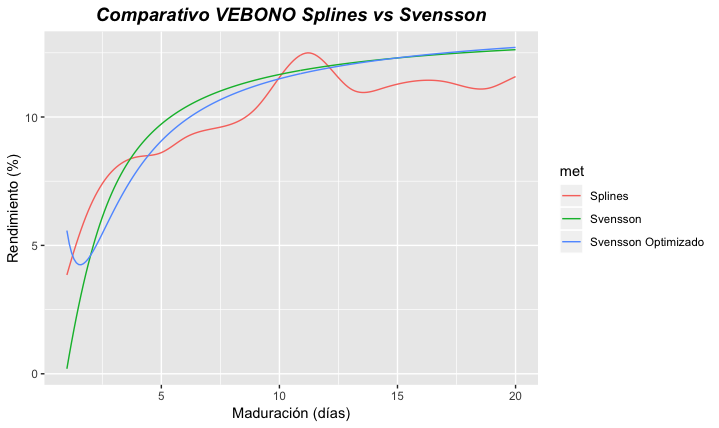
\includegraphics{images/Comparativo_vebono.png}}
\caption{Curva VEBONO Spline vs Svensson.}
\label{curva_spline_comp_veb}
\end{figure}


\newpage

\section{Conclusiones y Recomendaciones.}

\hspace{0.4cm}La curva de rendimiento es una herramienta muy importante al momento de obtener informaci\'on acerca de la tasa de inter\'es o rendimiento a una fecha determinada ya que dicha curva relaciona la maduraci\'on o fecha de vencimiento con el rendimiento. Una de las aplicaciones de esta curva, es que a partir de ella es posible obtener con facilidad el precio de un determinado instrumento, bono o t\'itulo, lo cual es de suma utilidad al momento de querer realizar alguna operaci\'on con el mismo, ya sea compra o venta del instrumento, ya que se tendr\'ia de antemano un precio referencial a partir del cual se puede tomar una decisi\'on. En otras palabras, la curva de rendimiento es una herramienta muy \'util al momento de tomar decisiones al realizar alguna inversi\'on.



\hspace{0.4cm} Para determinar dicha curva, varias metodolog\'ias han sido desarrolladas. Existen dos grandes enfoques que permiten su c\'alculo, el primer enfoque se basa en el uso de las metodolog\'ias param\'etricas de estimaci\'on, las cuales se caracterizan por estar atadas a ciertos par\'ametros, su uso es muy frecuete. Entre ellas, principalmente destacan la metodolog\'ia de Nelson y Siegel introducida en 1987 $[2]$, la metodolog\'ia de Svensson desarrollada en 1994 $[3]$, entre otras.


\hspace{0.4cm}Por otra parte, el segundo enfoque se centra en el uso de las metodolog\'ias no param\'etricas, las cuales se caracterizan por su flexibilidad ya que ellas no se encuentran atadas a ning\'un par\'ametro espec\'ifico sino que trabajan directamente con los datos suministrados. Entre ellas, destacan la metodolog\'ia de redes neuronales $[9]$, splines de polinomios $[6]$, splines c\'ubicos suavizados $[7]$, entre otras. En el presenta trabajo se aplica la \'ultima metodolog\'ia mencionada.


\hspace{0.4cm} La principal raz\'on de aplicar la metodolog\'ia de los splines c\'ubicos suavizados, fu\'e el balance que se obtiene como la misma, ya que ella presenta un equilibrio entre el ajuste a los datos y la suavidad de la curva resultante. Lo cual, es \'util cuando la data presenta mucho ruido ya que esta metodolog\'ia no interpola los valores ingresados sino que ajusta una curva suave que presenta el menor error de ajuste posible. En el presente trabajo se emple\'o la data de los Tif y Vebonos, instrumentos de la deuda p\'ublica nacional venezolana para el a\~no 2016 y 2017. Para ambos intrumentos se encontraron una cantidad aceptable de operaciones a partir de las cuales se calcu\'o el rendimiento y as\'i a partir de dichos valores calcular la curva de rendimientos. Una vez obtenida la curva, se procede a estimar los precios de los instrumentos involucrados.

\hspace{0.4cm} Al realizar la comparaciones de los precios te\'oricos obtenidos mediante las metodolog\'ias de Splines c\'ubicos de suavizado, Svensson no optimizado y Svensson optimizado, se puede afirmar que los precios te\'oricos que m\'as se asemejan a los precios promedio de cada tipo de instrumento, son aquellos obtenidos por la metodolog\'ia de Svensson optimizado. La raz\'on de esto se debe al proceso de optimizaci\'on que se lleva a cabo en dicha metodolog\'ia en donde se busca minimizar esta brecha. 


\hspace{0.4cm}De entrada esta es la principal fortaleza de esta metodolog\'ia, pero esto ocasiona tambi\'en que la misma dependa en demas\'ia de los precios promedio, lo cual en ocasiones no es del todo recomendable, puesto que en caso de considerar un precio promedio at\'ipico para alg\'un instrumento, la metodolog\'ia buscar\'a que los precios te\'oricos se asemejen a dicho precio promedio. De esta manera, la principal fortaleza de esta metodolog\'ia se puede convertir en una de sus debilidades.

\hspace{0.4cm} Teniendo en cuenta esto, la metodolog\'ia de los Splines c\'ubicos de suavizado tiene una ventaja ya que la misma no depende del comportamiento de los precios promedio, sino que la misma al ser una metodolog\'ia no param\'etrica se basa en trabajar directamente con los datos. Lo cual en este caso, es trabajar a partir del comportamiento de las operacione que se realicen con cada tipo de instrumento para un horizonte temporal dado.

\hspace{0.4cm} De esta manera, la metodolog\'ia de los Splines c\'ubicos de suavizado se considera una alternativa viable al momento de calcular los precios te\'oricos de los instrumentos de la deuda p\'ublica nacional para un tiempo determinado, con el fin de realizar la valoraci\'on de alg\'un portafolio y de esta manera saber si existen ganancia o perdidas por la tenencia de alg\'un instrumento. Como problema a resolver en futuros trabajos, se propone el c\'alculo del par\'ametro de suavizamiento de manera autom\'atica. 



